%!TEX root=masterproef.tex
\chapter{Achtergrond}
\label{chapter:achtergrond}

In dit hoofdstuk wordt het kader geschetst waarbinnen deze thesis op zoek gaat
naar antwoorden. Enerzijds wordt in sectie \ref{section:landscape} het
landschap van draadloze sensornetwerken in kaart gebracht: wat typeert en
onderscheid hen van andere netwerken? Waarom is het vaststellen van inbreuken
een belangrijk onderzoeksdomein?

Anderzijds wordt in sectie \ref{section:related} ingegaan op een groot aanbod
aan gerelateerd onderzoek. Een belangrijke doelstelling van deze thesis is het
in kaart brengen van de mogelijkheden en beperkingen betreffende reeds
beschreven methodes om inbreuken vast te stellen.

De verschillende beschreven methodes worden gecatalogeerd en gegroepeerd op
basis van verschillende eigenschappen. Op basis van dit overzicht wordt
vervolgens een inschatting gemaakt van de mogelijke dekking die kan bereikt
worden met de bestaande oplossingen.

Bij de beschrijving van de verschillende oplossingen zal tevens kritisch
nagegaan worden in hoeverre de oplossingen in een realistische situatie
effectief bijdragen tot het detecteren van inbreuken in het netwerk.

\section{Draadloze sensornetwerken}
\label{section:landscape}

\TODO

\section{Gerelateerd onderzoek}
\label{section:related}

\TODO

\subsection{Reputatie en vertrouwen}

De probleemstelling dat knopen in het netwerk elkaar niet langer kunnen
vertrouwen, zette verschillende onderzoekers aan tot het zoeken naar
oplossingen gebaseerd op reputatie en vertrouwen.

\cite{ganeriwal2008reputation} beschrijft een architectuur gebaseerd op
observaties door knopen van de acties van andere knopen in het kader van acties
van zichzelf of derde knopen. Figuur \ref{fig:reputation-cooperation} toont de
situaties die beschouwd worden: in \ref{fig:reputation-cooperative-node} zal
een co\"operatieve knoop (C) alle boodschappen die via hem verzonden worden
door een zendende knoop (Z) effectief doorsturen naar een verder gelegen
ontvangende knoop (O). De verzender van de boodschap, alsook andere naburige
knopen (B) kunnen deze actie vaststellen. In
\ref{fig:reputation-uncooperative-node} daarentegen zal een een
niet-co\"operatieve knoop (NC) deze boodschappen niet verder versturen of zelfs
aanpassen.

\begin{figure}
\centering
\begin{subfigure}{.49\textwidth}
\centering
\[ \entrymodifiers={-=+++[o][F-]}
 \xymatrix@!=0.75pc {
  Z \ar[dr] & *{}       & *{} & *{} \\
  *{}       & C \ar[rr] & *{} & O   \\
  B         & *{}       & *{} & *{} \\
 }
\]
\caption{Co\"operatieve knoop}
\label{fig:reputation-cooperative-node}
\end{subfigure}
\begin{subfigure}{.49\textwidth}
\centering
\[ \entrymodifiers={-=+++[o][F-]}
 \xymatrix@!=0.75pc {
  Z \ar[dr] & *{}       & *{} & *{} \\
  *{}       & NC        & *{} & O   \\
  B         & *{}       & *{} & *{} \\
 }
\]
\caption{Niet-co\"operatieve knoop}
\label{fig:reputation-uncooperative-node}
\end{subfigure}
\caption{Beschouwde situaties bij al dan niet co\"operatieve knopen.}
\label{fig:reputation-cooperation}
\end{figure}

Gegeven knopen $i$ en $j$, met $\alpha_j$, het aantal observaties van acties van
knoop $j$ dat als co\"operatief werd beschouwd, en $\beta_j$, het aantal niet
co\"operatieve acties, toont men aan dat de reputatie van knoop $j$ wordt
weergegeven door een beta distributie van $\alpha_j$ en $\beta_j$:

\begin{equation} \label{eq:reputation-beta}
R_{ij} \sim Beta(\alpha_j+1, \beta_j+1)
\end{equation}

Van deze reputatie kan vervolgens een vertrouwen bepaald worden van knoop $i$
ten opzichte van knoop $j$ als volgt: 

\begin{equation} \label{eq:reputation-trust}
\begin{array}{rcl}
T_{ij} & = & E(R_{ij}) \\
       & = & E(Beta(\alpha_j+1, \beta_j+1)) \\
       & = & \frac{\alpha_j+1}{\alpha_j+\beta_j+2} \\
\end{array}
\end{equation}

$\alpha_j$ en $\beta_j$ evolueren doorheen de tijd. Hierbij dienen enerzijds
nieuwe observaties binnen afzonderlijke tijdspannes beschouwd te worden, maar
moet ook een wegingsfactor toegepast worden op de oude waarden om er voor te
zorgen dat een historisch opgebouwd beeld niet dominant blijft en nieuwe
wijzigingen in het gedrag overstemt. Gegeven $r$ het aantal co\"operatieve
observaties in een bepaalde tijdspanne en $s$ het aantal niet-co\"operatieve
observaties in diezelfde tijdspanne worden de nieuwe waarden voor $\alpha_j$ en
$\beta_j$ gegeven door:

\begin{equation} \label{eq:reputation-update-direct}
\begin{array}{rcl}
\alpha^{new}_j & = & (w_{age} \times \alpha_j) + r \\
\beta^{new}_j  & = & (w_{age} \times \beta_j) + s \\
\end{array}
\end{equation}

Hierbij is $w_{age}$ een factor ($< 1$) die zorgt voor een afname van de
belangrijkheid van de oudere informatie.

Naast deze eigen directe observaties, kunnen ook indirecte observaties door
naburige knopen in beschouwing genomen worden. Voor zo'n naburige knoop, $k$,
zal een knoop $i$ eveneens een vertrouwen $T_{ik}$ kunnen bepalen op basis van
$\alpha_k$ en $\beta_k$. Knoop $k$ kan vervolgens zijn eigen informatie met
betrekking tot de reputatie van knoop $j$ kenbaar maken als $\alpha^k_j$ en
$\beta^k_j$. Knoop $i$ kan vervolgens zijn parameters bijwerken als volgt:

\begin{equation} \label{eq:reputation-update-indirect}
\begin{array}{rrcl}
& \alpha^{new}_j & = & \alpha_j + ( w^k_{rep} \times \alpha^k_j ) \\
& \beta^{new}_j  & = & \beta_j  + ( w^k_{rep} \times \beta^k_j )  \\
met \\
& w^k_{rep}      & = & \frac{2 \alpha_k}{(\beta_k+2) (\alpha^k_j+\beta^k_j+2)+2 \alpha_k} \\
\end{array}
\end{equation}

De factor $w^k_{rep}$ zorgt er voor dat de opname van indirecte informatie van
knoop $k$ in verhouding tot zijn reputatie zal gebeuren.

Enkele bijkomende regels beschermen tegen typische problemen gerelateerd aan
deze aanpak: een knoop accepteert slechts indirecte informatie van een andere,
indien deze knoop zelf als vertrouwd wordt beschouwd. Hierbij wordt een
drempelwaarde ($TH_{SHI}$) gehanteerd. Verder wordt enkel positieve informatie
uitgewisseld, om negatieve be\"invloeding te vermijden. Tot slot wordt tevens
alleen directe informatie uitgewisseld, om de onafhankelijkheid van de
informatie te garanderen.

De auteurs vermelden zelf een zeer belangrijk probleem: omdat knopen constant
moeten luisteren naar de acties van naburige knopen, moeten zij constant actief
zijn. Dit is een zeer nadelig uitgangspunt voor systemen die typisch trachten
zuinig om te springen met hun energie.

Maar de architectuur heeft ook inherente problemen en laat kwaadwillige
partijen toe om - mits kennis van de parameters - net onder de radar te
opereren. We illustreren dit met de simulatie zoals deze uitgevoerd werd door
de auteurs.

De evolutie van een volledige co\"operatieve of volledige niet-co\"operatieve
knoop wordt weergegeven in figuur \ref{fig:reputation-paper}. Een eigenschap
van het algoritme is dat pas na een tiental (louter positieve) observaties een
knoop de drempelwaarde van vertrouwen overschrijdt.

\begin{figure}[h]
\centering
\begin{subfigure}{.49\textwidth}
  \centering
  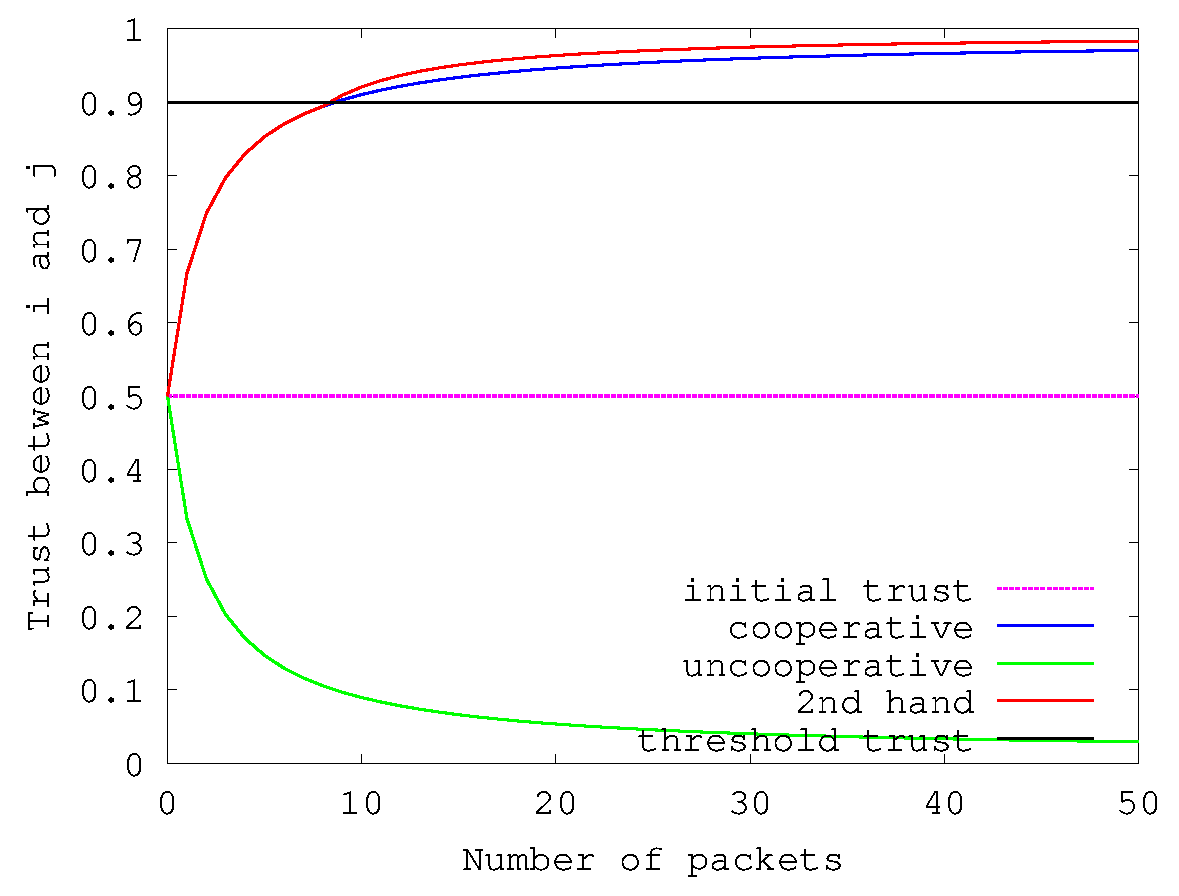
\includegraphics[width=.9\linewidth]{./resources/reputation-paper.eps}
  \caption{Co\"operatieve en niet-co\"operatieve knopen}
  \label{fig:reputation-paper}
\end{subfigure}
\begin{subfigure}{.49\textwidth}
  \centering
  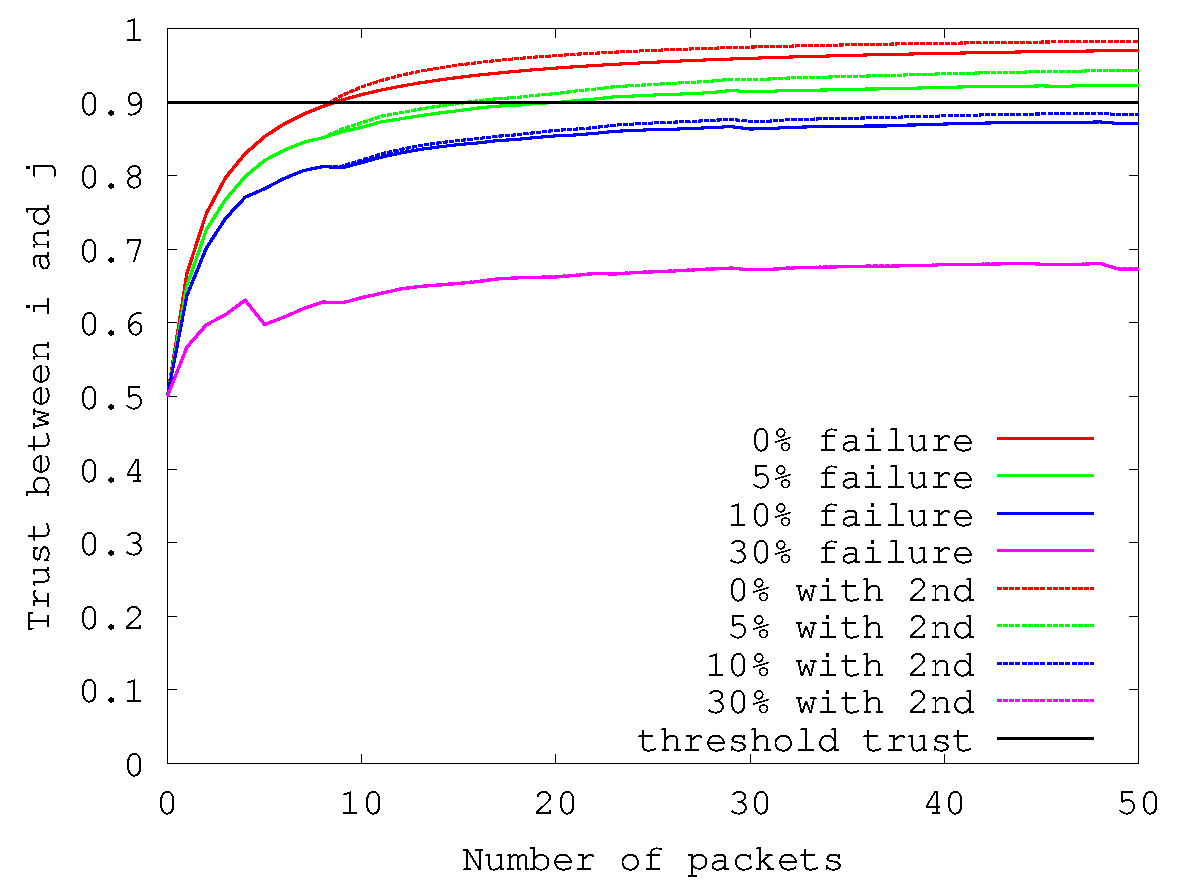
\includegraphics[width=.9\linewidth]{./resources/reputation-with-failure.eps}
  \caption{Falende knopen (100 simulaties)}
  \label{fig:reputation-with-failure}
\end{subfigure}
\caption{Impact van falende knopen op evolutie van vertrouwen.}
\label{fig:reputation-paper-with-failure}
\end{figure}

Deze eigenschap kan echter misbruikt worden zoals aangetoond wordt in figuur
\ref{fig:reputation-with-failure}. Stel dat een knoop $j$ te kampen heeft met
falende hardware, waardoor 5\% van zijn transmissies verloren gaan en daarom
ook niet opgemerkt kunnen worden door andere knopen.

We merken op dat deze knoop, zelfs met 5\% niet-co\"operatieve observaties, na
een twintigtal observaties toch boven de drempelwaarde uitkomt en door de
beschouwende knoop aanvaard wordt als betrouwbaar.

Vanuit een operationeel standpunt gezien is dit in eerste instantie een
positief effect. Indien een knoop \emph{slechts} 5\% faalt zal deze toch als
co\"operatief beschouwd worden en de goede werking van het netwerk niet
fundamenteel in het gedrang brengen - vanuit een inbraakdetectie oogpunt gezien.

Maar stel dat deze 5\% niet-co\"operatieve acties geen falen zijn en dat de
doorgestuurde boodschappen niet verloren gaan, maar met opzet lichtjes
gewijzigd worden. 5\% kan een significante vertekening van metingen van een
netwerk betekenen en zo de werking van het hele netwerk ondermijnen.

Figuur \ref{fig:reputation-malicious} gaat slechts een kleine stap verder en
toont het effect van falende (of malafide) knopen die pas falingen vertonen
nadat ze het vertrouwen hebben gekregen van een knoop. We merken op dat nu zelfs
10\% falingen zeer lang het vertrouwen kunnen behouden.

\begin{figure}[h]
 \centering
 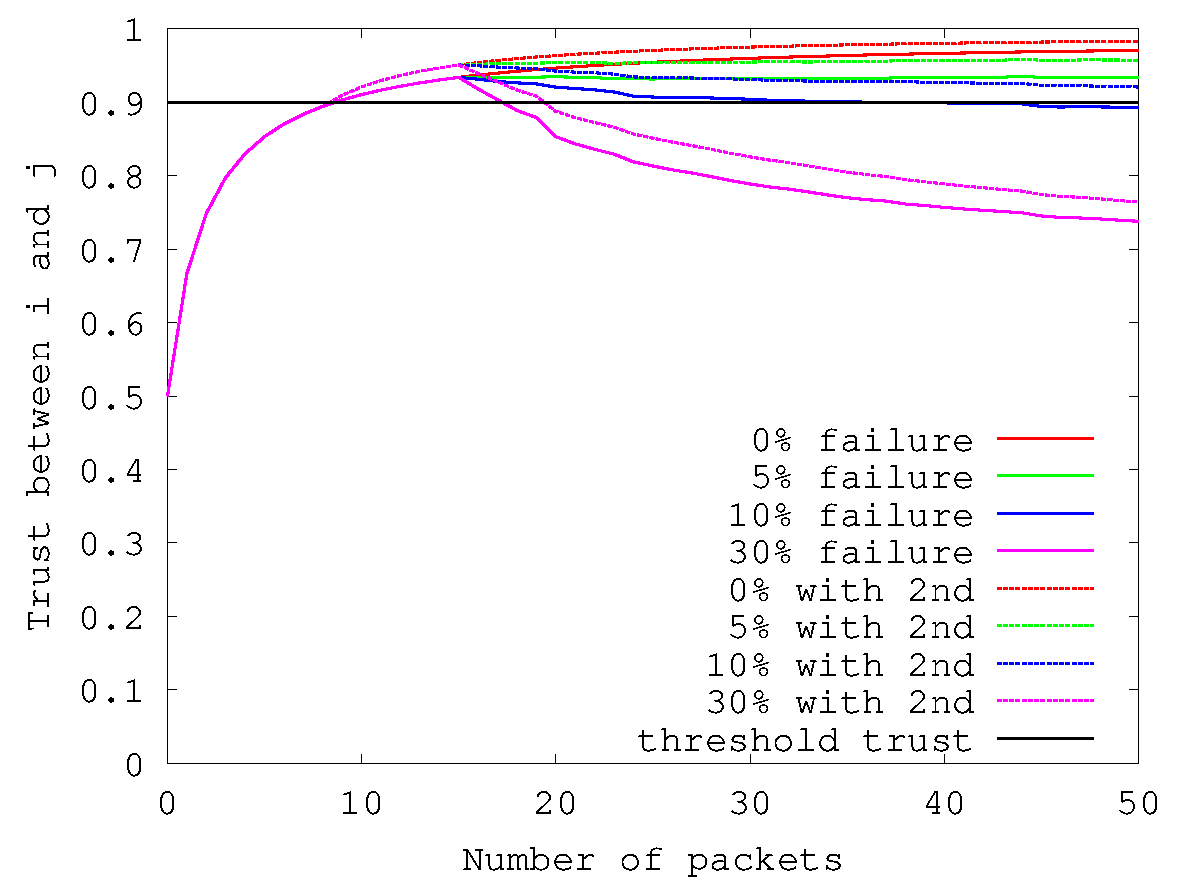
\includegraphics[width=.5\linewidth]{./resources/reputation-malicious.eps}
 \caption{Falende knopen met vertraging van 15 pakketten (100 simulaties)}
 \label{fig:reputation-malicious}
\end{figure}

Dit elementaire voorbeeld toont duidelijk aan dat het vaststellen van een
reputatie op basis van externe observaties een zeer delicaat onderwerp is dat
zeer gevoelig is voor manipulatie op basis van kennis van de interne
parameters. Dit laatste is dan weer net \'e\'en van d\'e problemen waar
draadloze sensornetwerken mee kampen omdat knopen vrij eenvoudig kunnen
weggenomen, ge\"inspecteerd, gewijzigd en teruggeplaatst worden.

\subsection{Co\"operatieve algoritmen}

Het detecteren van abnormaal gedrag, dat op zijn beurt een indicatie kan zijn
van een (poging tot) inbraak, door \'e\'en knoop is \'e\'en ding. Als netwerk
van knopen tot een consensus komen en met meer zekerheid een verdachte knoop
uitsluiten is een heel ander ding.

Een veel voorkomend onderwerp daarom is dat van co\"operatie tussen knopen om
in overleg te bepalen of en welke andere knoop uitgesloten moet worden uit het
netwerk. In \cite{krontiris2009cooperative} wordt hiertoe eerst langs een
theoretische weg gezocht naar de nodige en voldoende voorwaarden voor
inbraakdetectie. Vervolgens wordt er een praktisch omkaderend algoritme
voorgesteld om op co\"operatieve manier aan inbraak detectie te doen.

Zowel het theoretische model als het praktische algoritme vormen een
interessante bron van informatie. Het theoretische model kan helpen bij het
analyseren van andere co\"operatieve oplossingen en het praktische algoritme
biedt een algemeen raamwerk voor het implementeren van co\"operatieve
strategie\"en.

\subsubsection*{IDP}

Het theoretische model beschrijft het ``Intrusion Detection Problem'', IDP, aan
de hand van $S = \{ s_1, s_2, \dots s_n \}$, de set van sensoren in het netwerk,
$N(s)$, de set van buren van $s$ en $D(s)$, de set van knopen die door $s$
verdacht worden. Indien $|D(s)| = 1$, is de aanvaller ge\"identificeerd.

Enkele predicaten worden gedefinieerd als volgt: $source(q)$ geldt indien $q$
de aanvaller is, $honest(s) \iff \neg source(s)$, $expose_s(q) \iff D(s) = \{ q
\}$ ofwel $s$ verklaart dat $q$ de aanvaller is en $A(s) \iff D(s) \not= \{\}$
wat zoveel betekent als dat $s$ gealarmeerd is. De set van gealarmeerde buren
van een knoop $s$ wordt gedefinieerd als $AN(s) = \{ t | A(t) \wedge t \in N(s)
\}$ en de set van gealarmeerde buren die nuttig is voor een knoop $s$ wordt dan
uitgedrukt als $\tilde{AN}(q,s) = AN(q) \backslash \{s\}$.

Het IDP wordt vervolgens gedefinieerd als het vinden van een algoritme dat
voldoet aan de eigenschappen van correctheid: $\forall s \in S : honest(s)
\wedge expose_s(s') \implies A(s) \wedge source(s')$ en eindigheid: bij een
aanval zullen na een tijd alle eerlijke knopen in de gealarmeerde set een knoop
verdenken.

Twee condities worden voorgesteld: de ``Intrusion Detection Condition'' of IDC
en de ``Neighbourhood Conditions'' of NC. Indien aan minstens \'e\'en van deze
condities voldaan is, is het IDP oplosbaar.

De IDC wordt beschreven als $\forall p,q \in S : source(q) \implies
\tilde{AN}(p,q) \not= \tilde{AN}(q,p)$. Dit drukt uit dat geen enkele andere
knoop een zelfde gealarmeerde buurt kan hebben als de aanvaller.

De NC worden beschreven door ``\emph{alle buren van een aanvaller zijn
gealarmeerd}'' ($NC_1$) en ``\emph{indien twee of meer knopen verdacht zijn door
een meerderheid van knopen, hebben de eerlijke knopen niet-gealarmeerde buren}''
($NC_2$).

Figuur \ref{fig:idp-examples} illustreert het IDP en toepassing van IDC en NC
aan de hand van enkele voorbeelden:

\begin{figure}
\centering
\begin{subfigure}{.49\textwidth}
  \centering
\[ \entrymodifiers={}
 \xymatrix@!=0.75pc {
 *{}                                      & *{} & *-=++[o][F]{b} \ar@<0.7ex>[dll]\\
 *-=++[F]{a} \ar@<0.7ex>[urr] \ar@<0.7ex>[drr]& *{} & *{}                        \\
 *{}                                      & *{} & *-=++[o][F]{c} \ar@<0.7ex>[ull]\\
 }
\]
  \caption{}
  \label{fig:idp-examples-1}
\end{subfigure}
\begin{subfigure}{.49\textwidth}
  \centering
\[ \entrymodifiers={}
 \xymatrix@!=0.75pc {
 *{} & *{} & *{}                                      & *{} & *-=++[o][F]{b} \ar@<0.7ex>[dll] \ar[dd]\\
 *-=++[o][F]{d} \ar@<0.7ex>[rr] & *{} & *-=++[F]{a} \ar@<0.7ex>[ll] \ar@<0.7ex>[urr] \ar@<0.7ex>[drr]& *{} & *{} \\
 *{} & *{} & *{}                                      & *{} & *-=++[o][F]{c} \\
 }
\]
  \caption{}
  \label{fig:idp-examples-2}
\end{subfigure}
\caption{Voorbeelden van de toepassing van IDC en NC. Vierkante knopen zijn
aanvallers, omcirkelde knopen zijn gealarmeerd. $x \rightarrow y$ betekent dat
knoop $x$ knoop y verdenkt.}
\label{fig:idp-examples}
\end{figure}

De situatie in figuur \ref{fig:idp-examples-1} voldoet niet aan de IDC omdat
$\tilde{AN}(a,b) = \{c\} = \tilde{AN}(b,a)$. Maar in dit geval is wel voldaan
aan beide NC. Het IDP kan in dit geval opgelost worden aan de hand van een
deterministisch algoritme. Omdat er slechts \'e\'en knoop het hoogste aantal
verdenkingen op zijn naam heeft staan, kunnen knopen $b$ en $c$ eenvoudig
beslissen dat knoop $a$ de aanvaller is.

Figuur \ref{fig:idp-examples-2} toont een situatie waar de IDC wel voldaan is
want $\tilde{AN}(q,r) = \{s\} \not= \tilde{AN}(r,q) = \{\}$. Er zijn echter nu
twee knopen met een meerderheid aan verdenkingen: $a$ en $c$. Vanuit het
standpunt van knoop $b$ moet dus knoop $a$ of knoop $d$ valse aantijgingen
verspreiden. Als \'e\'en van deze knopen de aanvaller is, dan moet
$\tilde{AN}(a,d) \not= \tilde{AN}(d,a)$, anders is niet voldaan aan de IDC. Dit
impliceert tevens dat $\exists x : A(x) \wedge ( x \not\in N(a) \vee x \not\in
N(d) )$, ofwel dat er een knoop bestaat die gealarmeerd is, maar geen buur is
van de andere eerlijke knoop van de twee verdachte knopen. In dit geval zijn
knopen $b$ en $d$ inderdaad geen buren, maar beide verdenken knoop $a$.

\subsubsection*{Algoritme}

Naast een theoretisch model, introduceren \cite{krontiris2009cooperative}
tevens een algoritme dat kan dienen als raamwerk voor co\"operatieve
inbraakdetectie. Het algoritme bestaat uit vier tot vijf fasen: initialisatie,
stemming, publicatie van gebruikte sleutels, ontmaskeren van de aanvaller en
optioneel het inroepen van informatie uit de externe kring.

Tijdens de initialisatie fase krijgt elke knoop een unieke sleutel, $K_l$. Aan
de hand van deze sleutel wordt een \'e\'en-richtingsketting van langte $l$
gemaakt van sleutels door het toepassen van bv. SHA1 \cite{rfc:3174} hashing
toe te passen: $\{K_0, K_1, \dots K_{l-1}\}$ waarbij $\forall k \in [1..l] :
K_{k-1} = SHA1(K_k)$. Daarnaast worden ook naburige knopen gezocht tot twee
knopen ver en wordt sleutel $K_0$ gecommuniceerd aan al deze buren. De
volledige initialisatie fase wordt verondersteld te gebeuren zonder
mogelijkheid tot inbraken.

Tijdens de stemming brengen alle knopen een stem uit van de vorm $m_v(s),$ $
MAC_{K_j}(m_v(s))$. $m_v(s)$ bestaat uit een lijst van knopen die door knoop
$s$ beschouwd worden als mogelijke aanvallers, of uitgedrukt aan de hand van
het theoretische model: $m_v(s) = D(s)$. De $MAC_{K_j}()$ functie is een zgn.
\emph{Message Authentication Code} \cite{rfc:2104} en wordt meestal berekend
door het toepassen van een \'e\'en-richtings-hashfunctie toe te passen op de
boodschap. Typisch wordt er aan de boodschap een unieke, wederzijds gekende
identificatie toegevoegd, zodat de ontvanger van een boodschap deze
handtekening ook kan berekenen en vergelijken met het origineel. In dit geval
wordt $K_j$ gebruikt, waarbij $j$ de volgende indexwaarde krijg uit lijst van
beschikbare sleutels.

Een dergelijke boodschap kan op ogenblik van verzending door geen enkele andere
knoop gevalideerd worden. De enige sleutel die zij tot op dat ogenblik kennen
is de vorige en de vorige is net het resultaat van een SHA1 operatie op de
volgende. Dit betekent dat ook een mogelijke aanvaller niet in staat is om de
boodschap te wijzigen.

Pas wanneer de knopen elkaars stemmen hebben ontvangen, wordt de gebruikte
sleutel vrijgegeven in de publicatie fase. Op dit ogenblik kunnen de knopen de
eerder verstuurde stemmen valideren. Ze kunnen eerst controleren of de
gepubliceerde sleutel inderdaad de juiste is. Immers, door het toepassen van
SHA1 op deze sleutel, moeten zij de huidige gekende sleutel bekomen. Na
validatie van de nieuwe sleutel, kan ook de boodschap gevalideerd worden.

Nu alle knopen de stemmen van alle knopen ontvangen hebben en zeker zijn dat de
stemmen authentiek zijn, kan met \'e\'enzelfde algoritme door alle knopen de
aanvaller bepaald worden tijdens de ontmaskering fase.

Het is echter mogelijk dat er meerdere knopen zijn met eenzelfde aantal stemmen
zijn, iets dat typisch overeenkomt met een gelijke samenstelling van
gealarmeerde buren, wanneer de IDC niet kan gerealiseerd worden. Onder
voorbehoud dat aan de NC wel voldaan wordt, kan door het inroepen van de niet
gealarmeerde buren van de gealarmeerde knopen. Deze zullen op hun beurt nagaan
of de knopen die verdacht worden, buren zijn en dan aangeven dat zij hen
\emph{niet} verdenken. Aan de hand van deze informatie kunnen de eerder
gealarmeerde knopen hun beslissing verder staven.

Het algoritme is een betrekkelijk eenvoudig raamwerk voor een co\"operatieve
aanpak, waarbij knopen lokaal beslissen welke andere knopen ze verdenken en
vervolgens gedistribueerd, gezamenlijk trachten tot een consensus te komen
welke van de de verdachte knopen effectief de aanvaller is.

De kracht van dit raamwerk en het succes ervan hangt natuurlijk sterk af van de
lokale detectie mogelijkheden van de knopen en de accuraatheid hiervan.

\subsubsection*{Risico's}

Het voorbeeld in figuur \ref{fig:idp-examples-2} beslaat een zeer beperkte
scope. We moeten voorzichtig zijn om hier niet te snel tot conclusies te komen
die in een ruimere situatie misschien een totaal verkeerd beeld zouden kunnen
opleveren. Figuur \ref{fig:sinkhole-ripple} toont essentieel het zelfde
voorbeeld als dat van \ref{fig:idp-examples-2}, maar nu met meer knopen rondom
het initi\"ele voorbeeld.

Het routering algoritme is gebaseerd op de totale kost van het pad naar het
basisstation en komt daarmee overeen met het MultiHopLQI routering algoritme
beschreven in o.a. \cite{krontiris2008launching}. In dit werk wordt ook de zgn.
\emph{Sinkhole Attack} voorgesteld. We nemen deze aanval als voorbeeld.

\begin{figure}
\centering
\begin{subfigure}{.49\textwidth}
  \centering
\[ \entrymodifiers={-=++[o][F]}
 \xymatrix@!=0.75pc {
*{} & e \ar@{->}[l]_{100} & *{} & f \ar@{->}[ll]_{50}   & *{} \\
*{} & *{} & *{} &  *{} & b \ar@{->}[lu]_{35} \ar@{.}[ld]_{20} \ar@{.}[dd]^{30}  \\
*{} & d \ar@{->}[uu]^{75} \ar@{.}[dd]_{75}  & *{} &    a \ar@{->}[lluu]_{80} \ar@{.}[lldd]^{80} \ar@{.}[ll]_{50} & *{} \\
*{} & *{} & *{} &  *{} & c \ar@{.}[lu]^{20} \ar@{->}[ld]^{35} \\
*{} & h \ar@{->}[l]^{105}  & *{} &  g \ar@{->}[ll]^{50}  & *{} \\
  }
\]
  \caption{Initi\"ele topologie, routes en kosten}
  \label{fig:sinkhole-ripple-1}
\end{subfigure}
\begin{subfigure}{.49\textwidth}
  \centering
\[ \entrymodifiers={-=++[o][F]}
 \xymatrix@!=0.75pc {
*{} & e \ar@{->}[l]_{100} & *{} & f \ar@{->}[ll]_{50}   & *{} \\
*{} & *{} & *{} &  *{} & b \ar@{.}[lu]_{35} \ar@{~>}[ld]_{20} \ar@{.}[dd]^{30}  \\
*{} & *-=++[F]{d} \ar@{~>}[l]^{50} \ar@{.}[uu]^{75} \ar@{.}[dd]_{75}  & *{} &    a \ar@{.}[lluu]_{80} \ar@{.}[lldd]^{80} \ar@{~>}[ll]_{50} & *{} \\
*{} & *{} & *{} &  *{} & c \ar@{~>}[lu]^{20} \ar@{.}[ld]^{35} \\
*{} & h \ar@{->}[l]^{105}  & *{} &  g \ar@{->}[ll]^{50}  & *{} \\
  }
\]
  \caption{Knoop $d$ kondigt ``betere'' route aan.}
  \label{fig:sinkhole-ripple-2}
\end{subfigure}
\caption{Voorbeeld van het theoretische risico dat kan leiden tot een verkeerde
identificatie van de echte aanvaller.}
\label{fig:sinkhole-ripple}
\end{figure}

Stel dat knoop $d$ een \emph{Sinkhole Attack} uitvoert door een zeer lage kost
te adverteren. Hierdoor zal knoop $a$ geneigd zijn om zijn route aan te passen.
Hierdoor zal deze op zijn beurt een veel voordeligere route adverteren en
zullen ook knopen $b$ en $c$ hun route wijzigen en nu hun gegevens via knoop
$a$ versturen.

Ten gevolge van deze route updates is het mogelijk dat een lokale detector voor
de \emph{Sinkhole Attack} op knopen $a$ en $b$ zal in werking treden. Hierbij
kunnen de knopen slechts hun volledige buurt beschuldigen, omdat het niet
mogelijk is om te detecteren wie de valse boodschappen effectief verstuurd
heeft. Indien de aanvallende knoop $d$ nu ook selectief zijn naburige knoop $a$
beschuldigd, bekomen we dezelfde situatie als in figuur
\ref{fig:idp-examples-2}, echter nu met mogelijk een verkeerd
ge\"identificeerde aanvaller.

Dit voorbeeld is, net zoals de vele andere beschreven voorbeelden, uitermate
specifiek en dient louter ter illustratie van het fragiele karakter van een
co\"operatief algoritme. Desalniettemin bieden de concepten en het omkaderende
algoritme ge\"introduceerd in \cite{krontiris2009cooperative} een goed
uitgangspunt om te hanteren bij het beschrijven en implementeren van inbraak
detectie mechanismen.

\TODO

\cite{castelluccia2009difficulty,krauss2007detecting,seshadri2008sake,maerien2012famos,aschenbruck2012security,afzal2012difisec,yue2012novel,kuang2010snds,blilat2012wireless,ramesh2012wireless,valero2012di,perrig2004security,zhang2000intrusion,djenouri2005survey,yu2008framework,rassam2011novel,da2005decentralized,kachirski2003effective,li2008group,mishra2004intrusion,krontiris2008lidea,ioannis2007towards,soliman2012comparative,wang2011integrated,zhijie2012intrusion}
